\documentclass{article}

% ============================================================
% INFR11269 Machine Learning Systems — Coursework Report
% Academic year 2026/27
%
% This coursework uses the official ICLR 2027 LaTeX style.
%
% IMPORTANT FORMAT RULES
% - Do not edit iclr2027_conference.sty.
% - Do not change page geometry, text width/height, base font size,
%   or line spacing.
% - Do not enable \iclrfinalcopy.
% - Normal content packages are fine if they do not alter the report format.
%
% Main-body page limit: six pages.
% References and Appendix do NOT count toward the main-body page limit.
% Reviewers are not obliged to read Appendix at all. Please put your main content
% in the main body.
% 
% AI policy:
% Academic integrity is an underlying principle of research and academic practice.
% All submitted work is expected to be your own, including any material you have
% generated yourself with the assistance of AI tools such as ELM, ChatGPT,
% Bing Chat, Claude, Google Gemini, or any other automated assistance.
% For all such material you must make prominent explicit acknowledgement and
% explain clearly what you have done in the AI declaration section.
% This includes using AI to directly generate text, code, figures or similar
% or to complete other tasks. In all cases, you remain entirely responsible
% for the material you produce.
% ============================================================

\usepackage{iclr2027_conference,times}
\usepackage{hyperref}
\usepackage{url}
\hypersetup{hidelinks}
\usepackage{booktabs}
\usepackage{graphicx}
\usepackage{amsmath}
\usepackage{amssymb}
\usepackage{float}
\usepackage{tikz}


% The official ICLR archive includes math_commands.tex. It is optional:
%%%%% NEW MATH DEFINITIONS %%%%%

\usepackage{amsmath,amsfonts,bm}

% Mark sections of captions for referring to divisions of figures
\newcommand{\figleft}{{\em (Left)}}
\newcommand{\figcenter}{{\em (Center)}}
\newcommand{\figright}{{\em (Right)}}
\newcommand{\figtop}{{\em (Top)}}
\newcommand{\figbottom}{{\em (Bottom)}}
\newcommand{\captiona}{{\em (a)}}
\newcommand{\captionb}{{\em (b)}}
\newcommand{\captionc}{{\em (c)}}
\newcommand{\captiond}{{\em (d)}}

% Highlight a newly defined term
\newcommand{\newterm}[1]{{\bf #1}}


% Figure reference, lower-case.
\def\figref#1{figure~\ref{#1}}
% Figure reference, capital. For start of sentence
\def\Figref#1{Figure~\ref{#1}}
\def\twofigref#1#2{figures \ref{#1} and \ref{#2}}
\def\quadfigref#1#2#3#4{figures \ref{#1}, \ref{#2}, \ref{#3} and \ref{#4}}
% Section reference, lower-case.
\def\secref#1{section~\ref{#1}}
% Section reference, capital.
\def\Secref#1{Section~\ref{#1}}
% Reference to two sections.
\def\twosecrefs#1#2{sections \ref{#1} and \ref{#2}}
% Reference to three sections.
\def\secrefs#1#2#3{sections \ref{#1}, \ref{#2} and \ref{#3}}
% Reference to an equation, lower-case.
\def\eqref#1{equation~\ref{#1}}
% Reference to an equation, upper case
\def\Eqref#1{Equation~\ref{#1}}
% A raw reference to an equation---avoid using if possible
\def\plaineqref#1{\ref{#1}}
% Reference to a chapter, lower-case.
\def\chapref#1{chapter~\ref{#1}}
% Reference to an equation, upper case.
\def\Chapref#1{Chapter~\ref{#1}}
% Reference to a range of chapters
\def\rangechapref#1#2{chapters\ref{#1}--\ref{#2}}
% Reference to an algorithm, lower-case.
\def\algref#1{algorithm~\ref{#1}}
% Reference to an algorithm, upper case.
\def\Algref#1{Algorithm~\ref{#1}}
\def\twoalgref#1#2{algorithms \ref{#1} and \ref{#2}}
\def\Twoalgref#1#2{Algorithms \ref{#1} and \ref{#2}}
% Reference to a part, lower case
\def\partref#1{part~\ref{#1}}
% Reference to a part, upper case
\def\Partref#1{Part~\ref{#1}}
\def\twopartref#1#2{parts \ref{#1} and \ref{#2}}

\def\ceil#1{\lceil #1 \rceil}
\def\floor#1{\lfloor #1 \rfloor}
\def\1{\bm{1}}
\newcommand{\train}{\mathcal{D}}
\newcommand{\valid}{\mathcal{D_{\mathrm{valid}}}}
\newcommand{\test}{\mathcal{D_{\mathrm{test}}}}

\def\eps{{\epsilon}}


% Random variables
\def\reta{{\textnormal{$\eta$}}}
\def\ra{{\textnormal{a}}}
\def\rb{{\textnormal{b}}}
\def\rc{{\textnormal{c}}}
\def\rd{{\textnormal{d}}}
\def\re{{\textnormal{e}}}
\def\rf{{\textnormal{f}}}
\def\rg{{\textnormal{g}}}
\def\rh{{\textnormal{h}}}
\def\ri{{\textnormal{i}}}
\def\rj{{\textnormal{j}}}
\def\rk{{\textnormal{k}}}
\def\rl{{\textnormal{l}}}
% rm is already a command, just don't name any random variables m
\def\rn{{\textnormal{n}}}
\def\ro{{\textnormal{o}}}
\def\rp{{\textnormal{p}}}
\def\rq{{\textnormal{q}}}
\def\rr{{\textnormal{r}}}
\def\rs{{\textnormal{s}}}
\def\rt{{\textnormal{t}}}
\def\ru{{\textnormal{u}}}
\def\rv{{\textnormal{v}}}
\def\rw{{\textnormal{w}}}
\def\rx{{\textnormal{x}}}
\def\ry{{\textnormal{y}}}
\def\rz{{\textnormal{z}}}

% Random vectors
\def\rvepsilon{{\mathbf{\epsilon}}}
\def\rvtheta{{\mathbf{\theta}}}
\def\rva{{\mathbf{a}}}
\def\rvb{{\mathbf{b}}}
\def\rvc{{\mathbf{c}}}
\def\rvd{{\mathbf{d}}}
\def\rve{{\mathbf{e}}}
\def\rvf{{\mathbf{f}}}
\def\rvg{{\mathbf{g}}}
\def\rvh{{\mathbf{h}}}
\def\rvu{{\mathbf{i}}}
\def\rvj{{\mathbf{j}}}
\def\rvk{{\mathbf{k}}}
\def\rvl{{\mathbf{l}}}
\def\rvm{{\mathbf{m}}}
\def\rvn{{\mathbf{n}}}
\def\rvo{{\mathbf{o}}}
\def\rvp{{\mathbf{p}}}
\def\rvq{{\mathbf{q}}}
\def\rvr{{\mathbf{r}}}
\def\rvs{{\mathbf{s}}}
\def\rvt{{\mathbf{t}}}
\def\rvu{{\mathbf{u}}}
\def\rvv{{\mathbf{v}}}
\def\rvw{{\mathbf{w}}}
\def\rvx{{\mathbf{x}}}
\def\rvy{{\mathbf{y}}}
\def\rvz{{\mathbf{z}}}

% Elements of random vectors
\def\erva{{\textnormal{a}}}
\def\ervb{{\textnormal{b}}}
\def\ervc{{\textnormal{c}}}
\def\ervd{{\textnormal{d}}}
\def\erve{{\textnormal{e}}}
\def\ervf{{\textnormal{f}}}
\def\ervg{{\textnormal{g}}}
\def\ervh{{\textnormal{h}}}
\def\ervi{{\textnormal{i}}}
\def\ervj{{\textnormal{j}}}
\def\ervk{{\textnormal{k}}}
\def\ervl{{\textnormal{l}}}
\def\ervm{{\textnormal{m}}}
\def\ervn{{\textnormal{n}}}
\def\ervo{{\textnormal{o}}}
\def\ervp{{\textnormal{p}}}
\def\ervq{{\textnormal{q}}}
\def\ervr{{\textnormal{r}}}
\def\ervs{{\textnormal{s}}}
\def\ervt{{\textnormal{t}}}
\def\ervu{{\textnormal{u}}}
\def\ervv{{\textnormal{v}}}
\def\ervw{{\textnormal{w}}}
\def\ervx{{\textnormal{x}}}
\def\ervy{{\textnormal{y}}}
\def\ervz{{\textnormal{z}}}

% Random matrices
\def\rmA{{\mathbf{A}}}
\def\rmB{{\mathbf{B}}}
\def\rmC{{\mathbf{C}}}
\def\rmD{{\mathbf{D}}}
\def\rmE{{\mathbf{E}}}
\def\rmF{{\mathbf{F}}}
\def\rmG{{\mathbf{G}}}
\def\rmH{{\mathbf{H}}}
\def\rmI{{\mathbf{I}}}
\def\rmJ{{\mathbf{J}}}
\def\rmK{{\mathbf{K}}}
\def\rmL{{\mathbf{L}}}
\def\rmM{{\mathbf{M}}}
\def\rmN{{\mathbf{N}}}
\def\rmO{{\mathbf{O}}}
\def\rmP{{\mathbf{P}}}
\def\rmQ{{\mathbf{Q}}}
\def\rmR{{\mathbf{R}}}
\def\rmS{{\mathbf{S}}}
\def\rmT{{\mathbf{T}}}
\def\rmU{{\mathbf{U}}}
\def\rmV{{\mathbf{V}}}
\def\rmW{{\mathbf{W}}}
\def\rmX{{\mathbf{X}}}
\def\rmY{{\mathbf{Y}}}
\def\rmZ{{\mathbf{Z}}}

% Elements of random matrices
\def\ermA{{\textnormal{A}}}
\def\ermB{{\textnormal{B}}}
\def\ermC{{\textnormal{C}}}
\def\ermD{{\textnormal{D}}}
\def\ermE{{\textnormal{E}}}
\def\ermF{{\textnormal{F}}}
\def\ermG{{\textnormal{G}}}
\def\ermH{{\textnormal{H}}}
\def\ermI{{\textnormal{I}}}
\def\ermJ{{\textnormal{J}}}
\def\ermK{{\textnormal{K}}}
\def\ermL{{\textnormal{L}}}
\def\ermM{{\textnormal{M}}}
\def\ermN{{\textnormal{N}}}
\def\ermO{{\textnormal{O}}}
\def\ermP{{\textnormal{P}}}
\def\ermQ{{\textnormal{Q}}}
\def\ermR{{\textnormal{R}}}
\def\ermS{{\textnormal{S}}}
\def\ermT{{\textnormal{T}}}
\def\ermU{{\textnormal{U}}}
\def\ermV{{\textnormal{V}}}
\def\ermW{{\textnormal{W}}}
\def\ermX{{\textnormal{X}}}
\def\ermY{{\textnormal{Y}}}
\def\ermZ{{\textnormal{Z}}}

% Vectors
\def\vzero{{\bm{0}}}
\def\vone{{\bm{1}}}
\def\vmu{{\bm{\mu}}}
\def\vtheta{{\bm{\theta}}}
\def\va{{\bm{a}}}
\def\vb{{\bm{b}}}
\def\vc{{\bm{c}}}
\def\vd{{\bm{d}}}
\def\ve{{\bm{e}}}
\def\vf{{\bm{f}}}
\def\vg{{\bm{g}}}
\def\vh{{\bm{h}}}
\def\vi{{\bm{i}}}
\def\vj{{\bm{j}}}
\def\vk{{\bm{k}}}
\def\vl{{\bm{l}}}
\def\vm{{\bm{m}}}
\def\vn{{\bm{n}}}
\def\vo{{\bm{o}}}
\def\vp{{\bm{p}}}
\def\vq{{\bm{q}}}
\def\vr{{\bm{r}}}
\def\vs{{\bm{s}}}
\def\vt{{\bm{t}}}
\def\vu{{\bm{u}}}
\def\vv{{\bm{v}}}
\def\vw{{\bm{w}}}
\def\vx{{\bm{x}}}
\def\vy{{\bm{y}}}
\def\vz{{\bm{z}}}

% Elements of vectors
\def\evalpha{{\alpha}}
\def\evbeta{{\beta}}
\def\evepsilon{{\epsilon}}
\def\evlambda{{\lambda}}
\def\evomega{{\omega}}
\def\evmu{{\mu}}
\def\evpsi{{\psi}}
\def\evsigma{{\sigma}}
\def\evtheta{{\theta}}
\def\eva{{a}}
\def\evb{{b}}
\def\evc{{c}}
\def\evd{{d}}
\def\eve{{e}}
\def\evf{{f}}
\def\evg{{g}}
\def\evh{{h}}
\def\evi{{i}}
\def\evj{{j}}
\def\evk{{k}}
\def\evl{{l}}
\def\evm{{m}}
\def\evn{{n}}
\def\evo{{o}}
\def\evp{{p}}
\def\evq{{q}}
\def\evr{{r}}
\def\evs{{s}}
\def\evt{{t}}
\def\evu{{u}}
\def\evv{{v}}
\def\evw{{w}}
\def\evx{{x}}
\def\evy{{y}}
\def\evz{{z}}

% Matrix
\def\mA{{\bm{A}}}
\def\mB{{\bm{B}}}
\def\mC{{\bm{C}}}
\def\mD{{\bm{D}}}
\def\mE{{\bm{E}}}
\def\mF{{\bm{F}}}
\def\mG{{\bm{G}}}
\def\mH{{\bm{H}}}
\def\mI{{\bm{I}}}
\def\mJ{{\bm{J}}}
\def\mK{{\bm{K}}}
\def\mL{{\bm{L}}}
\def\mM{{\bm{M}}}
\def\mN{{\bm{N}}}
\def\mO{{\bm{O}}}
\def\mP{{\bm{P}}}
\def\mQ{{\bm{Q}}}
\def\mR{{\bm{R}}}
\def\mS{{\bm{S}}}
\def\mT{{\bm{T}}}
\def\mU{{\bm{U}}}
\def\mV{{\bm{V}}}
\def\mW{{\bm{W}}}
\def\mX{{\bm{X}}}
\def\mY{{\bm{Y}}}
\def\mZ{{\bm{Z}}}
\def\mBeta{{\bm{\beta}}}
\def\mPhi{{\bm{\Phi}}}
\def\mLambda{{\bm{\Lambda}}}
\def\mSigma{{\bm{\Sigma}}}

% Tensor
\DeclareMathAlphabet{\mathsfit}{\encodingdefault}{\sfdefault}{m}{sl}
\SetMathAlphabet{\mathsfit}{bold}{\encodingdefault}{\sfdefault}{bx}{n}
\newcommand{\tens}[1]{\bm{\mathsfit{#1}}}
\def\tA{{\tens{A}}}
\def\tB{{\tens{B}}}
\def\tC{{\tens{C}}}
\def\tD{{\tens{D}}}
\def\tE{{\tens{E}}}
\def\tF{{\tens{F}}}
\def\tG{{\tens{G}}}
\def\tH{{\tens{H}}}
\def\tI{{\tens{I}}}
\def\tJ{{\tens{J}}}
\def\tK{{\tens{K}}}
\def\tL{{\tens{L}}}
\def\tM{{\tens{M}}}
\def\tN{{\tens{N}}}
\def\tO{{\tens{O}}}
\def\tP{{\tens{P}}}
\def\tQ{{\tens{Q}}}
\def\tR{{\tens{R}}}
\def\tS{{\tens{S}}}
\def\tT{{\tens{T}}}
\def\tU{{\tens{U}}}
\def\tV{{\tens{V}}}
\def\tW{{\tens{W}}}
\def\tX{{\tens{X}}}
\def\tY{{\tens{Y}}}
\def\tZ{{\tens{Z}}}


% Graph
\def\gA{{\mathcal{A}}}
\def\gB{{\mathcal{B}}}
\def\gC{{\mathcal{C}}}
\def\gD{{\mathcal{D}}}
\def\gE{{\mathcal{E}}}
\def\gF{{\mathcal{F}}}
\def\gG{{\mathcal{G}}}
\def\gH{{\mathcal{H}}}
\def\gI{{\mathcal{I}}}
\def\gJ{{\mathcal{J}}}
\def\gK{{\mathcal{K}}}
\def\gL{{\mathcal{L}}}
\def\gM{{\mathcal{M}}}
\def\gN{{\mathcal{N}}}
\def\gO{{\mathcal{O}}}
\def\gP{{\mathcal{P}}}
\def\gQ{{\mathcal{Q}}}
\def\gR{{\mathcal{R}}}
\def\gS{{\mathcal{S}}}
\def\gT{{\mathcal{T}}}
\def\gU{{\mathcal{U}}}
\def\gV{{\mathcal{V}}}
\def\gW{{\mathcal{W}}}
\def\gX{{\mathcal{X}}}
\def\gY{{\mathcal{Y}}}
\def\gZ{{\mathcal{Z}}}

% Sets
\def\sA{{\mathbb{A}}}
\def\sB{{\mathbb{B}}}
\def\sC{{\mathbb{C}}}
\def\sD{{\mathbb{D}}}
% Don't use a set called E, because this would be the same as our symbol
% for expectation.
\def\sF{{\mathbb{F}}}
\def\sG{{\mathbb{G}}}
\def\sH{{\mathbb{H}}}
\def\sI{{\mathbb{I}}}
\def\sJ{{\mathbb{J}}}
\def\sK{{\mathbb{K}}}
\def\sL{{\mathbb{L}}}
\def\sM{{\mathbb{M}}}
\def\sN{{\mathbb{N}}}
\def\sO{{\mathbb{O}}}
\def\sP{{\mathbb{P}}}
\def\sQ{{\mathbb{Q}}}
\def\sR{{\mathbb{R}}}
\def\sS{{\mathbb{S}}}
\def\sT{{\mathbb{T}}}
\def\sU{{\mathbb{U}}}
\def\sV{{\mathbb{V}}}
\def\sW{{\mathbb{W}}}
\def\sX{{\mathbb{X}}}
\def\sY{{\mathbb{Y}}}
\def\sZ{{\mathbb{Z}}}

% Entries of a matrix
\def\emLambda{{\Lambda}}
\def\emA{{A}}
\def\emB{{B}}
\def\emC{{C}}
\def\emD{{D}}
\def\emE{{E}}
\def\emF{{F}}
\def\emG{{G}}
\def\emH{{H}}
\def\emI{{I}}
\def\emJ{{J}}
\def\emK{{K}}
\def\emL{{L}}
\def\emM{{M}}
\def\emN{{N}}
\def\emO{{O}}
\def\emP{{P}}
\def\emQ{{Q}}
\def\emR{{R}}
\def\emS{{S}}
\def\emT{{T}}
\def\emU{{U}}
\def\emV{{V}}
\def\emW{{W}}
\def\emX{{X}}
\def\emY{{Y}}
\def\emZ{{Z}}
\def\emSigma{{\Sigma}}

% entries of a tensor
% Same font as tensor, without \bm wrapper
\newcommand{\etens}[1]{\mathsfit{#1}}
\def\etLambda{{\etens{\Lambda}}}
\def\etA{{\etens{A}}}
\def\etB{{\etens{B}}}
\def\etC{{\etens{C}}}
\def\etD{{\etens{D}}}
\def\etE{{\etens{E}}}
\def\etF{{\etens{F}}}
\def\etG{{\etens{G}}}
\def\etH{{\etens{H}}}
\def\etI{{\etens{I}}}
\def\etJ{{\etens{J}}}
\def\etK{{\etens{K}}}
\def\etL{{\etens{L}}}
\def\etM{{\etens{M}}}
\def\etN{{\etens{N}}}
\def\etO{{\etens{O}}}
\def\etP{{\etens{P}}}
\def\etQ{{\etens{Q}}}
\def\etR{{\etens{R}}}
\def\etS{{\etens{S}}}
\def\etT{{\etens{T}}}
\def\etU{{\etens{U}}}
\def\etV{{\etens{V}}}
\def\etW{{\etens{W}}}
\def\etX{{\etens{X}}}
\def\etY{{\etens{Y}}}
\def\etZ{{\etens{Z}}}

% The true underlying data generating distribution
\newcommand{\pdata}{p_{\rm{data}}}
% The empirical distribution defined by the training set
\newcommand{\ptrain}{\hat{p}_{\rm{data}}}
\newcommand{\Ptrain}{\hat{P}_{\rm{data}}}
% The model distribution
\newcommand{\pmodel}{p_{\rm{model}}}
\newcommand{\Pmodel}{P_{\rm{model}}}
\newcommand{\ptildemodel}{\tilde{p}_{\rm{model}}}
% Stochastic autoencoder distributions
\newcommand{\pencode}{p_{\rm{encoder}}}
\newcommand{\pdecode}{p_{\rm{decoder}}}
\newcommand{\precons}{p_{\rm{reconstruct}}}

\newcommand{\laplace}{\mathrm{Laplace}} % Laplace distribution

\newcommand{\E}{\mathbb{E}}
\newcommand{\Ls}{\mathcal{L}}
\newcommand{\R}{\mathbb{R}}
\newcommand{\emp}{\tilde{p}}
\newcommand{\lr}{\alpha}
\newcommand{\reg}{\lambda}
\newcommand{\rect}{\mathrm{rectifier}}
\newcommand{\softmax}{\mathrm{softmax}}
\newcommand{\sigmoid}{\sigma}
\newcommand{\softplus}{\zeta}
\newcommand{\KL}{D_{\mathrm{KL}}}
\newcommand{\Var}{\mathrm{Var}}
\newcommand{\standarderror}{\mathrm{SE}}
\newcommand{\Cov}{\mathrm{Cov}}
% Wolfram Mathworld says $L^2$ is for function spaces and $\ell^2$ is for vectors
% But then they seem to use $L^2$ for vectors throughout the site, and so does
% wikipedia.
\newcommand{\normlzero}{L^0}
\newcommand{\normlone}{L^1}
\newcommand{\normltwo}{L^2}
\newcommand{\normlp}{L^p}
\newcommand{\normmax}{L^\infty}

\newcommand{\parents}{Pa} % See usage in notation.tex. Chosen to match Daphne's book.

\DeclareMathOperator*{\argmax}{arg\,max}
\DeclareMathOperator*{\argmin}{arg\,min}

\DeclareMathOperator{\sign}{sign}
\DeclareMathOperator{\Tr}{Tr}
\let\ab\allowbreak


\title{Optimising CUDA speech recognition kernels by data reusing}

% Keep this line unchanged.
\author{Anonymous coursework submission}

% Keep this COMMENTED OUT.
% Review mode is part of the coursework format and is checked automatically.
% \iclrfinalcopy

\begin{document}

\maketitle

% Course-specific template fingerprint. Keep this line unchanged.
\lhead{Under review as a report for UoE 26/27 Sem1 INFR11269: Machine Learning Systems}

% Keep this COMMENTED OUT.
% \begin{abstract}
% \end{abstract}

% ============================================================
% REPORT CONTENT GUIDANCE

% The structure below is RECOMMENDED, not mandatory.
% You may rename, merge, split, or reorder sections if another structure
% better communicates your investigation.

% Regardless of section titles, the report should make it easy to find:
%   1. the problem, motivation, and relevant system context;
%   2. the supplied baseline and your substantive technical work;
%   3. experimental methodology, metrics, and controlled comparisons;
%   4. results covering task/system quality AND relevant system cost;
%   5. analysis of why the results occur, limitations, and conclusions.
% Well organized report would result in better scores.

% Depth is preferred over implementing many unrelated features.
% ============================================================

\section{Introduction}
\label{sec:introduction}

In the course system, a spoken question is first transcribed by automatic speech recognition (ASR). A retrieval system uses the transcript to find relevant documents, and a language model answers using those documents. The user waits for all three steps. In our investigation, we primarily forcused on the optimisation of ASR kernels. 

We have noticed that in the provided GEMM and attention kernel, which all together takes over 99\% of time when running on the test audio (see appendix~\ref{app:profile}, the data can be further reused by increasing the work allocated to each unit. This is supposed to have a large influence to the final performance as pointed out in the Roofline model\citep{williams2009roofline}.
But this modification also faces the trade-off of resource cost, degree of parallelism, and computation waste.

Therefore, we explore two questions with experiments: a) Can we lower latency by giving each thread or block more work so it can reuse more data? b) When a larger tile leaves slots empty or creates too few blocks, how much can a kernel designed for that shape recover?

\section{System and Technical Approach}
\label{sec:approach}
The course supplies the GLM-ASR-Nano model, its Python code, model weights, and the retrieval and answer pipeline \citep{course-asr,course-rag}. Python passes GPU tensor addresses and the CUDA stream to our compiled kernel library. The audio encoder processes the recording once. The text decoder generates the transcript a token at a time and recomputes its sequence at each step, because this model keeps no cache of previous keys and values. Its final linear layer scores vocabulary entries from just the last position. 

The focus of our exploration is on the optimisation for ASR, therefore, we have changed the ASR kernel in the pipeline while keeping the other codes of RAG fixed.

\subsection{Answers to the ASR questions}
\label{sec:asr-questions}

\paragraph{Task 1 (Q3). Why rotate both queries and keys in one launch?}
Fusing the query and key rotations saves 396 kernel launches per transcription. Each launch incurs work to submit and start the kernel. The model calls rotary position embedding (RoPE) 396 times, so separate launches for \(q\) and \(k\) would require \(2\times396=792\) launches. Their pairs can be rotated independently, so threads in one grid can process both arrays with the same arithmetic and memory accesses.

\paragraph{Task 2 (Q2). How does subtracting the maximum stabilise softmax?}
\texttt{expf(100.0f)} returns \(+\infty\) in float32. Because the largest finite float32 value is \((2-2^{-23})2^{127}\approx3.40\times10^{38}\), while \(e^{100}\approx2.69\times10^{43}\). Subtracting the row maximum prevents exponential overflow and preserves the exact softmax probabilities.  With \(m=\max_i x_i\), every \(x_i-m\le0\) and at least one is zero, so the shifted sum of exponentials lies between \(1\) and \(513\), the row length. In exact arithmetic, \(e^{x_i-m}/\sum_j e^{x_j-m}=e^{x_i}/\sum_j e^{x_j}\) because \(e^{-m}\) cancels.

\paragraph{Task 3 (Q1). How many input values does each matrix kernel request?}
At \(M=N=K=1024\), the naive kernel requests \(2{,}147{,}483{,}648\) floats from global memory and our Tiled-16 kernel requests \(134{,}217{,}728\), ignoring caches. Each of the \(1024^2\) naive outputs reads an input and a weight at each of \(1024\) dot-product steps, for \(2\cdot1024^3\) loads. Tiled-16 launches \(64^2\) blocks, each taking \(64\) steps along \(K\) and loading one \(16\times16\) tile from \(X\) and one from \(W\) per step. That is \(64^2\cdot64\cdot2\cdot16^2\) loads. In section~\ref{sec:results}, experiments A and B test how this reuse trade-off changes with wider tiles and different shapes.

\paragraph{Task 4 (Q4). How often is each encoder key loaded?}
With \texttt{ATTN\_WARPS=4}, each key of one encoder head is requested from global memory 375 times per layer. GPU resources and the number of blocks available to run in parallel limit how far we can increase the warp count. Every encoder query attends to every key. Each block handles up to \(w\) queries, one per warp, and loads each key once. This gives \(\lceil1500/w\rceil\) requests per key, or \(\lceil1500/4\rceil=375\) at four warps and \(\lceil1500/16\rceil=94\) at sixteen. A block uses \(32w\) threads and stores \(wd\) query values in shared memory for head dimension \(d\). More threads, registers and shared memory can limit how many blocks fit on a multiprocessor. A larger \(w\) also creates fewer blocks and can leave more idle warps in the last block. In our experiment C1, it is checked whether fewer loads actually reduce latency.

\subsection{Modification to the kernels}

\paragraph{More outputs per GEMM thread.}
We enlarge the output tile to reuse more data. The costs of which are more registers and shared memory, fewer blocks to run in parallel, and extra work in partial tiles. We keep 256 threads per block and give each thread a \(4\times4\) patch of outputs and 16 partial sums. This grows the block's tile from \(16\times16\) to \(64\times64\). At each position along \(K\), a full \(t\times t\) tile loads \(t\) inputs and \(t\) weights for \(t^2\) multiply-adds. Global-memory requests per multiply-add fall from \(2/16\) to \(2/64\), a \(75\%\) reduction. We expect the saving to pay off on large encoder projections. A \(1500\times1280\) output still gives \(24\times20=480\) mostly full blocks for 16 multiprocessors.

\paragraph{Two exceptions to 4-by-4.}
Figure~\ref{fig:gemm-dispatch} shows how we select a kernel from the matrix shape. The vocabulary projection has \(M=1\), so only one row of a 64-row tile is useful. The single-row path assigns a warp to each output column. Its lanes read consecutive weights along \(K\) and sum their partial results within the warp. The decoder's narrow key and value projections can leave too few blocks to use the slice. For \(M=64,N=512\), the smaller output tiles of Tiled-32 yield 32 blocks, up from eight with 4-by-4 on our 16-multiprocessor slice.

\begin{figure}[H]
\centering
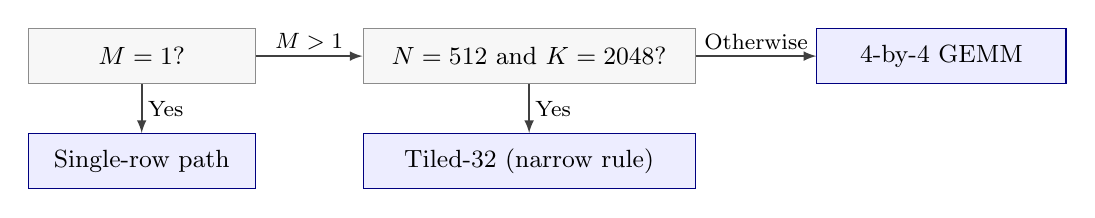
\begin{tikzpicture}[
  box/.style={rectangle, draw, minimum height=20pt, inner sep=3pt, font=\small},
  test/.style={box, draw=black!45, fill=black!3},
  path/.style={box, draw=blue!50!black, fill=blue!7},
  branch/.style={->, >=latex, semithick, draw=black!75},
  note/.style={font=\footnotesize, inner sep=2pt}
]
\node[test, minimum width=82pt] (single) at (0,0) {\(M=1\)?};
\node[test, minimum width=120pt] (narrow) at (140pt,0) {\(N=512\) and \(K=2048\)?};
\node[path, minimum width=90pt] (general) at (289pt,0) {4-by-4 GEMM};
\node[path, minimum width=82pt] (vector) at (0,-38pt) {Single-row path};
\node[path, minimum width=120pt] (tiled) at (140pt,-38pt) {Tiled-32 (narrow rule)};
\draw[branch] (single) -- node[note, above] {\(M>1\)} (narrow);
\draw[branch] (narrow) -- node[note, above] {Otherwise} (general);
\draw[branch] (single) -- node[note, right] {Yes} (vector);
\draw[branch] (narrow) -- node[note, right] {Yes} (tiled);
\end{tikzpicture}
\caption{GEMM dispatch by output rows \(M\), output columns \(N\), and dot-product length \(K\).}
\label{fig:gemm-dispatch}
\end{figure}

\paragraph{More queries per attention block.}
We change the number of warps per block from four to 16. As Task 4 shows (Section~\ref{sec:asr-questions}), that takes the encoder from 375 to 94 load requests per key or value per head per layer, about \(75\%\) fewer. Each block grows from 128 to 512 threads and must hold more query data. The long encoder still has more blocks per head than the slice has multiprocessors, so we expect the added reuse to pay off there. Short sequences offer fewer blocks, and a partial final block can leave more warps idle. We keep the key--value tile size, online softmax and decoder mask fixed.

\section{Experimental Methodology}
\label{sec:methodology}

The completed course implementation is our system baseline, with \(16\times16\) GEMM output tiles (\emph{Tiled-16}) for all the linear layer and four attention warps. The later part of this report also refers to this baseline as \emph{Original}. Each comparison used a single teaching-cluster allocation with an NVIDIA H200 MIG \texttt{1g.18gb} slice (16 streaming multiprocessors), CUDA 12.8 and float32 ASR under PyTorch 2.10.0+cu128.

\paragraph{A. Change the general GEMM layout.}
Each block in the baseline GEMM computes a 16 tile of the output matrix, with each of its threads computes 1 element. We made experiments by testing square tiles of width 8 and 32 (\emph{Tiled-8} and \emph{Tiled-32}) and per-thread layouts with \(2\times2\), \(2\times4\) and \(4\times4\) outputs per thread (\emph{2-by-2}, \emph{2-by-4}, \emph{4-by-4}). We timed each layout on the same model-shaped tensors, then on the course's 3.5-second \texttt{test\_audio.wav}. 

\paragraph{B. Test the GEMM exceptions.}
To test the edge of this benefits of \emph{4-by-4} layout, we further tested different kernel's performance on different matrix shapes. 
We first varied M and N around tile boundaries and calculated block counts and operand requests from the dimensions. 
Then, for matrix with \(M=1\), we held the shape and operands fixed and timed Tiled-16, 4-by-4, and the single-row specific GEMM kernel. We used the number of vocabulary calls in the reference recording to estimate the impact of the per-call saving. For \(N=512,K=2048,M>1\), we varied \(M\) and compared 4-by-4 with Tiled-32, the kernel selected by the narrow rule. A separate \(M=2\) case explicitly exercised the rule against a CPU reference and under memory, race and synchronisation checks. The course GEMM suite covers other shapes.

\paragraph{C1. Vary attention warps per block.}
The attention kernel can be optimised under the similar idea. As is calculated in section~\ref{sec:asr-questions}, each key and value will be requested \(\lceil1500/\texttt{ATTN\_WARPS}\rceil\) times, so increasing this value should theoretically reduce time of data transmission.
We timed 1, 2, 8 and 16 warps on the same tensors while keeping the 32-key tiles fixed. Also, we used model shapes and synthetic lengths near tile boundaries, then counted tile visits to interpret the timings.

\textbf{C2.} In addition, to check the performance when the previous strategies are combined, we conducted another round of experiment. Here we compared the result of enabling the Tiled-32 narrow rule only, 16 warps only, and applying both. The general GEMM and single-row path stayed fixed. We compared the combined saving against the sum of the individual savings.

\paragraph{D. Run the full request with all changes enabled.}
We compiled the baseline and \emph{Final} from the same source and verified the loaded library in each request. Final uses 4-by-4 GEMM kernel, the single-row specific kernel, narrow matrix's Tiled-32 kernel and 16 attention warps. We split the 125 development recordings into three groups by duration and fixed a random sample of ten per group (seed 21). Sampled durations were 3.700--4.825, 4.950--6.075 and 6.200--8.425 seconds. After two practice requests per version, we ran three pairs per recording, randomising query order and which version ran first. Each request recomputed the transcript and called ELM live. The model weights, CPU \texttt{enc\_a} encoder, exact top-five retrieval, prompt builder and ELM settings (EuroLLM-22B-Instruct-2512, temperature 0.1) were fixed. Client retries were disabled.

\paragraph{Timing and checks for for the experiments.}
For test on isolated kernels, we ran five warm-up calls, followed by seven CUDA-event measurements of 20 calls each on preloaded tensors. We report the median time per call. Repeated access to one set of weights can favour caching compared with switching weights in the model. Numerical checks used double-precision CPU references or float32 cuBLAS for large matrix products. For the reference recording in A and C2, each of three model processes ran three warm-up transcriptions per configuration and ten timed transcriptions per configuration in randomly interleaved order. Model latency measures synchronised generation from prepared GPU tensors. Extra transcriptions recorded per-operation GPU event totals outside the timed trials. We checked the generated tokens and the reference transcript, and ran the course test suites.

For the RAG systems-cost, the measures were core ASR latency (synchronised model generation) and full request latency (audio input through answer return). We timed the ASR worker round trip, local query and retrieval steps, and the remote call. The worker also logged audio preparation time. Both measures exclude one-time startup and loading. We took the median of the paired time differences and ratios within each query, then across queries. We resampled queries 2,000 times for a 95\% interval on the median saving. We retained slow trials, logged feature shapes and token counts, and profiled one clip per duration group. We checked exact agreement of tokens, transcripts, rankings, context and prompts. For embeddings and scores we used absolute and relative tolerances of \(10^{-6}\) and \(10^{-5}\). We also measured Recall@5 against the course relevance labels.

\section{Results and Analysis}
\label{sec:results}

\subsection{General GEMM gains and limits}

Table~\ref{tab:gemm-model} shows the result of experiment A.
For a square output tile of width \(t\), let \(a=\lceil M/t\rceil\) and \(b=\lceil N/t\rceil\). The grid has \(ab\) blocks. Each row of \(X\) is read for each column tile, and each row of \(W\) for each row tile, so a kernel issues \(R=K(Mb+Na)\) operand elements. This counts valid operand requests before caching. A larger tile can lower \(R\) while still leaving enough blocks to keep the device busy on the encoder products. 4-by-4 gives the lowest model latency. Its drop in profiled linear time nearly matches the drop in model latency, consistent with the large gains on encoder products.

\begin{table}[H]
\centering
\caption{Experiment A. Median ASR latency on the reference recording, separately profiled linear time, and selected encoder kernel times. The single-row path and attention settings are fixed in the model comparison.}
\label{tab:gemm-model}
\small
\begin{tabular}{@{}lrrrrrr@{}}
\toprule
 & Tiled-16 & Tiled-8 & Tiled-32 & 2-by-2 & 2-by-4 & 4-by-4 \\
\midrule
ASR (s) & 5.942 & 8.258 & 5.506 & 4.626 & 3.798 & 3.382 \\
Linear profile (s) & 4.923 & -- & -- & -- & -- & 2.363 \\
Encoder query (ms) & 5.256 & -- & -- & -- & -- & 1.940 \\
Encoder FF expansion (ms) & 21.128 & -- & -- & -- & -- & 7.825 \\
Encoder FF contraction (ms) & 21.367 & -- & -- & -- & -- & 7.959 \\
\bottomrule
\end{tabular}
\end{table}

\subsection{Shape-specific GEMM}

On the small grid (Table~\ref{tab:gemm}), larger tiles cut operand requests but leave more multiprocessors idle. Timing worsens despite fewer requests. On the wider output, the extra row adds a band of blocks. Those blocks load another copy of the weights for each column tile while computing mostly empty output slots. Requests increase by \(50.8\%\) and latency by \(50.0\%\). The increase in requests and the extra block work both offer explanations.

\begin{table}[H]
\centering
\caption{Experiment B. Median GEMM time in ms. Calculated counts describe the work launched and valid operand requests before caching. The single-row estimate multiplies the kernel saving by the vocabulary call count.}
\label{tab:gemm}
\small
\begin{tabular}{@{}llrrrr@{}}
\toprule
 & Shape \((M,N,K)\) & Tiled-16 & 4-by-4 & Tiled-32 & Single-row \\
\midrule
B & \((32,256,2048)\) & 0.0478 & 0.1636 & -- & -- \\
B & \((64,2048,2048)\) & 0.6102 & 0.3038 & -- & -- \\
B & \((65,2048,2048)\) & 0.7500 & 0.4559 & -- & -- \\
B & \((1,59264,2048)\) & 4.0578 & 5.8120 & -- & 0.8865 \\
B & \((64,512,2048)\) & -- & 0.1690 & 0.1261 & -- \\
B & \((65,512,2048)\) & -- & 0.1691 & 0.1852 & -- \\
\bottomrule
\end{tabular}

\smallskip
\begin{tabular}{@{}lrr@{}}
\toprule
Calculated check & Before & After \\
\midrule
B: Small grid, Tiled-16 to 4-by-4 (blocks / million requests) & 32 / 2.097 & 4 / 0.786 \\
B: 4-by-4 at \(M=64\) to 65, \(N=2048\) (blocks / million requests) & 32 / 8.389 & 64 / 12.648 \\
\quad Change in requests / latency & & \(+50.8\% / +50.0\%\) \\
\quad Valid row slots & 100\% & 50.8\% \\
B: Narrow projection at \(M=64\), 4-by-4 to Tiled-32 (blocks) & 8 & 32 \\
\quad At \(M=65\) (blocks) & 16 & 48 \\
B: Vocabulary estimate (calls / saving) & & 13 / 41.2\,ms \\
\bottomrule
\end{tabular}
\end{table}

For the vocabulary projection, the single-row path avoids computing unused rows. Its local gain has limited reach. The call-count estimate in Table~\ref{tab:gemm} is small beside the general GEMM saving and assumes that the isolated per-call gain carries over to the model.

For the narrow projection, Tiled-32 provides more blocks when 4-by-4 launches too few to use the whole slice. Adding a row gives 4-by-4 enough blocks to reach every multiprocessor in principle. Tiled-32 already had enough, and its additional block band brings extra work. This offers a reason for the crossover without treating the calculated grid size as measured occupancy. The narrow rule covers both row counts. Its value depends on the mix of calls in the model, which we showed later in the combination result.

\subsection{Attention work at sequence boundaries}

With \(Q\) queries and \(w\) warps, each head has \(\lceil Q/w\rceil\) blocks. Every encoder block reads all key--value tiles. For causal attention with equal query and key lengths, block \(b\) (counting from one) visits \(\lceil \min(bw,Q)/s\rceil\) tiles of width \(s\). Table~\ref{tab:attn-length} sums these visits across blocks. Encoder latency falls less than the visit count, consistent with the query arithmetic that still has to run.

At the causal boundary, the last query adds a block that visits every tile, including the new one. The same addition is proportionally larger for the wider block, which also has more idle query warps. At length 65, the 16-warp setting still visits fewer tiles (9 versus 15 per head) yet takes longer. The short encoder case shows the same limit. Block resources and the available parallel work matter alongside reuse.

\begin{table}[H]
\centering
\caption{Experiment C1. Median kernel times and calculated key--value tile visits per query head. Visits include partial tiles. The causal tests have equal query and key lengths.}
\label{tab:attn-length}
\small
\begin{tabular}{@{}lr@{\hspace{1em}}rrr@{\hspace{1em}}rrr@{}}
\toprule
 & & \multicolumn{3}{c}{Latency (ms)} & \multicolumn{3}{c}{Tile visits} \\
\cmidrule(lr){3-5}\cmidrule(l){6-8}
Workload & Length & 4 warps & 8 warps & 16 warps & 4 & 8 & 16 \\
\midrule
Encoder & 1500 & 29.862 & 24.242 & 22.601 & 17,625 & 8,836 & 4,418 \\
Short encoder-style & 32 & 0.0206 & 0.0162 & 0.0168 & 8 & 4 & 2 \\
Causal decoder & 64 & 0.0793 & 0.0561 & 0.0496 & 24 & 12 & 6 \\
Causal boundary & 65 & 0.0943 & 0.0683 & 0.0712 & 27 & 15 & 9 \\
\bottomrule
\end{tabular}
\end{table}

\subsection{Combination of individual strategies}

Subtracting both individual savings from the control predicts a time close to the combined measurement (Table~\ref{tab:asr}). The narrow rule saves linear time, and extra warps save attention time. The profile supports approximate additivity on this recording. The trials produced the same tokens and expected transcript. Appendices~\ref{app:profile} and~\ref{app:checks} give the profiles and successful course tests.

\begin{table}[H]
\centering
\caption{Experiment C2. Model medians and savings relative to its four-warp control. Profile savings are differences in separate GPU-event medians. Positive values mean less time.}
\label{tab:asr}
\small
\begin{tabular}{@{}lrrrrr@{}}
\toprule
Configuration & Model (ms) & Saved (ms) & Saved (\%) & Linear (ms) & Attn. (ms) \\
\midrule
4 warps, narrow rule off & 3372.00 & -- & -- & -- & -- \\
4 warps, narrow rule on & 3336.70 & 35.30 & 1.05 & 35.61 & \(-0.05\) \\
16 warps, narrow rule off & 3129.04 & 242.96 & 7.21 & 0.76 & 242.37 \\
16 warps, narrow rule on & 3093.89 & 278.11 & 8.25 & 36.67 & 242.36 \\
Additive prediction & 3093.74 & 278.26 & -- & -- & -- \\
\bottomrule
\end{tabular}
\end{table}

\subsection{RAG full request}

If only core ASR changes, the predicted full-request mean is \(\widehat{T}_F=T_O-A_O+A_F\), where \(T\) is mean full-request time and \(A\) is mean core ASR time. Table~\ref{tab:rag} compares prediction and measurement. The remote call takes nearly as long in both versions, which dilutes the ASR speedup. The observed mean exceeds the prediction because other local steps took longer. The paired interval supports a saving for this cohort.

\begin{table}[H]
\centering
\caption{Experiment D. Medians and paired measures are aggregated by query. Mean speedup is the ratio of overall means. Intervals give 95\% bootstrap bounds on median paired savings.}
\label{tab:rag}
\small
\begin{tabular}{@{}lrrrrr@{}}
\toprule
Metric & Original (s) & Final (s) & Speedup & Saved (s) & Interval (s) \\
\midrule
Core ASR & 7.865 & 3.983 & \(1.985\times\) & 3.932 & [3.437, 4.401] \\
Full request & 12.729 & 8.440 & \(1.461\times\) & 3.760 & [3.230, 4.341] \\
\midrule
Core ASR (mean) & 8.41 & 4.21 & -- & -- & -- \\
Other local steps (mean) & 0.57 & 0.81 & -- & -- & -- \\
Remote answer call (mean) & 4.99 & 4.98 & -- & -- & -- \\
Full request (mean) & 13.97 & 9.99 & \(1.40\times\) & -- & -- \\
Mean if only ASR changes & 13.97 & 9.78 & \(1.43\times\) & -- & -- \\
\bottomrule
\end{tabular}
\end{table}

\begin{table}[H]
\centering
\caption{Experiment D. Workload, regression and output checks. Encoder positions are from a separate profile of one clip per group. Positive paired savings mean Final was faster.}
\label{tab:rag-checks}
\small
\begin{tabular}{@{}lrrr@{}}
\toprule
Duration group & Output tokens per clip & Encoder positions & ASR speedup \\
\midrule
Short & 10--16 & 1,500 & \(1.872\times\) \\
Medium & 14--19 & 1,500 & \(1.989\times\) \\
Long & 17--26 & 1,500 & \(2.174\times\) \\
\bottomrule
\end{tabular}

\smallskip
\begin{tabular}{@{}lr@{}}
\toprule
Query or stage check & Result \\
\midrule
Queries faster in Final (ASR / full request) & 30 of 30 / 29 of 30 \\
Regressing query, paired median saving & \(-6.36\) s \\
Slowest Final repeat: preparation / encoding / ELM & 11.25 / 13.31 / 7.68 s \\
Exact match of tokens, transcript, ranking, context and prompt & 30/30 queries \\
Recall@5 (Original / Final) & 40.2\% / 40.2\% \\
\bottomrule
\end{tabular}
\end{table}

In the regressing query's slowest Final repeat, audio preparation and query encoding each took longer than the remote call (Table~\ref{tab:rag-checks}). The cause of this local delay remains unknown.

Long clips produced more tokens with the same feature size and profiled encoder lengths. Extra tokens add repeated decoder work without a key/value cache, which can increase the gain from faster kernels. Duration and decoder workload vary together here.

Embeddings and retrieval scores agreed within tolerance. Matching rankings and prompts show that the same evidence reached ELM. Recall@5 shows how much labelled evidence was retrieved. Transcription error against human references and answer quality remain open.

\section{Discussion and Conclusion}
\label{sec:conclusion}

The experiments prove the effectiveness of our optimsation strategies. Larger GEMM tiles and more attention queries per block sped up the operations that dominated ASR. With the single-row path and attention settings fixed, 4-by-4 reduced model latency by \(43\%\) on the reference recording. On the development set, the final configuration gave paired speedups of \(1.98\times\) for core ASR and \(1.46\times\) for full requests, with identical transcripts and retrieval rankings.

Although larger tiles and blocks use more resources, leave fewer blocks to schedule, and can waste work on partial tiles, the experiments show that these edge cases are overweighed by the gains from main workload. These changes required local edits to the CUDA kernels and a short GEMM dispatch rule, which also proves the cost-efficiency of our improvement.

Certain limitations also exist in our result. For example, all of our GPU measurements used the same H200 MIG slice configuration, but the best tile size and warp count may differ on GPUs with different caches and resources per multiprocessor. Also, although CUDA events show how long a kernel runs, the contributions of memory traffic, cache reuse and concurrent work remain uncertain. In the future investigation, we can repeat the shape comparisons on a different GPU and use a kernel profiler to measure device-memory traffic, cache hit rates and active warps, which can help reveal how broadly our conclusion applies.

% References are excluded from the main-body page limit.
\bibliography{references}
\bibliographystyle{iclr2027_conference}

% Put your Appendix here if needed. Comment out if you don't need it.
\appendix
\section{ASR profile records}
\label{app:profile}
\paragraph{General matrix comparison.}
The Tiled-16 control used the single-row path and four attention warps. All four course test suites passed on the same GPU allocation. The excerpt shows one transcription profiled with all CUDA kernels enabled using the course benchmark.

\begin{verbatim}
GPU: NVIDIA H200 MIG 1g.18gb (sm_90)
run 1: 5944.9 ms  (13 tokens)
GPU time per operation, one transcription (5943.8 ms in kernels):
  operation    runs on    calls   total ms   share
  linear       cuda        2757     4923.4   82.8%
  attention    cuda         396      996.1   16.8%
Transcription: Concord returned to its place amidst the tents.
Status: PASS
\end{verbatim}

\paragraph{Combined configuration.}
The combined configuration ran in a separate allocation of the same H200 MIG slice type. The table gives the median GPU event time per operation for one transcription across three model processes. Its course test results are in Appendix~\ref{app:checks}.

\begin{center}
\begin{tabular}{@{}lrr@{}}
\toprule
Operation & Calls & Median total event time (ms) \\
\midrule
\texttt{im2col} & 2 & 0.314 \\
\texttt{linear} & 2757 & 2324.838 \\
\texttt{layernorm} & 65 & 3.945 \\
\texttt{rope} & 396 & 5.409 \\
\texttt{attention} & 396 & 746.568 \\
\texttt{embedding} & 13 & 0.420 \\
\texttt{rmsnorm} & 741 & 6.428 \\
\texttt{silu\_mul} & 364 & 5.735 \\
\texttt{softmax} & 13 & 1.819 \\
\bottomrule
\end{tabular}
\end{center}


\clearpage
\section{Course test results}
\label{app:checks}
All cases below passed for the combined configuration, using the same GPU allocation as its operation profile. Times and errors are from the course test log.
\par\noindent\textbf{GPU.} \texttt{nvidia-smi -L} reported an NVIDIA H200 with a \texttt{MIG 1g.18gb} slice. The CUDA test reported 16 multiprocessors, target \texttt{sm\_90}.
\begin{center}
\begin{tabular}{@{}llrr@{}}
\toprule
Task & Passing case & Max. abs. error & Time (ms) \\
\midrule
1. RoPE & Tiny, 2 batches and 3 tokens & \(1.08\times 10^{-7}\) & 0.002 \\
 & odd sizes, partial rotation & \(1.08\times 10^{-7}\) & 0.002 \\
 & Audio encoder, partial rotation & \(1.93\times 10^{-7}\) & 0.063 \\
 & Text decoder, GQA 16/4 & \(1.64\times 10^{-7}\) & 0.007 \\
\addlinespace
2. Reductions & rmsnorm, one short row & \(8.27\times 10^{-8}\) & 0.002 \\
 & rmsnorm, odd cols & \(3.68\times 10^{-7}\) & 0.003 \\
 & rmsnorm, text decoder & \(4.35\times 10^{-7}\) & 0.005 \\
 & layernorm, odd cols (example) & \(3.91\times 10^{-7}\) & 0.004 \\
 & layernorm, audio encoder & \(5.42\times 10^{-7}\) & 0.059 \\
 & softmax, one short row & \(1.11\times 10^{-8}\) & 0.002 \\
 & softmax, odd cols & \(1.88\times 10^{-9}\) & 0.003 \\
 & softmax, large inputs ($\pm100$) & \(1.89\times 10^{-8}\) & 0.004 \\
 & softmax, all negative (-200..-150) & \(1.69\times 10^{-8}\) & 0.003 \\
 & softmax, vocabulary row (59264) & \(8.13\times 10^{-11}\) & 0.098 \\
 & softmax, 64 x 4096 & \(9.84\times 10^{-10}\) & 0.010 \\
\addlinespace
3. GEMM & tiny 3 x 5, K = 7 & \(9.76\times 10^{-9}\) & 0.003 \\
 & odd sizes 37 x 100, K = 33, bias & \(1.55\times 10^{-7}\) & 0.006 \\
 & odd sizes, bias + GELU & \(7.70\times 10^{-7}\) & 0.014 \\
 & Decoder query projection & \(1.14\times 10^{-5}\) & 0.305 \\
 & Decoder gate projection & \(0.00\times 10^{0}\) & 0.685 \\
 & Decoder down projection & \(3.72\times 10^{-5}\) & 0.903 \\
 & Vocabulary, last token & \(1.43\times 10^{-6}\) & 0.886 \\
 & Encoder query projection & \(1.01\times 10^{-5}\) & 1.938 \\
 & First encoder feed-forward layer with GELU & \(6.92\times 10^{-7}\) & 7.818 \\
 & Second convolution via matrix multiply & \(2.57\times 10^{-5}\) & 5.985 \\
\addlinespace
4. Attention & tiny, one tile (4 queries, 5 keys) & \(8.15\times 10^{-8}\) & 0.006 \\
 & several tiles, peaky scores & \(4.97\times 10^{-7}\) & 0.018 \\
 & GQA 4 heads / 2 kv heads & \(1.30\times 10^{-7}\) & 0.009 \\
 & causal, seq\_q = seq\_k & \(5.16\times 10^{-7}\) & 0.025 \\
 & causal, 5 new queries, 37 keys & \(1.78\times 10^{-7}\) & 0.010 \\
 & causal, one new query & \(3.39\times 10^{-7}\) & 0.024 \\
 & Text decoder, causal GQA 16/4 & \(5.21\times 10^{-7}\) & 0.050 \\
 & Audio encoder, 20 heads & \(2.68\times 10^{-7}\) & 22.601 \\
\bottomrule
\end{tabular}
\end{center}

% Keep this line unchanged.
\newpage

% Academic integrity is an underlying principle of research and academic practice.
% All submitted work is expected to be your own, including any material you have
% generated yourself with the assistance of AI tools such as ELM, ChatGPT,
% Bing Chat, Claude, Google Gemini, or any other automated assistance.
% For all such material you must make prominent explicit acknowledgement and
% explain clearly what you have done in this section.
% This includes using AI to directly generate text, code, figures or similar
% or to complete other tasks. In all cases, you remain entirely responsible
% for the material you produce.
\section*{AI declaration}
We completed all the required code blanks in the baseline CUDA kernels and implemented part of the optimisations and experimental code. We chose the research topic, prepared the report outline, and developed its main technical content and analysis.

We used OpenAI Codex for guidance on the baseline kernels and to check our implementation. Codex also helped refine the experiments and develop test scripts. For the report, we used Codex to revise parts of the text, adjust the LaTeX formatting, and create figures and tables. We take responsibility for the submitted code, results, and report.

% Please put the information of your group here without changing the format.
% This page will be deleted when the report is distributed for reviewing.
\section*{Group information}
Group ID: [MLS-0081]

Information of group member A:
\begin{itemize}
    \item Name: [Runqiu Yi]
    \item UUN: [S2955206]
\end{itemize}

Uncomment and complete if the group has two members.
Information of group member B:
\begin{itemize}
    \item Name: [Alexandru-David Gogu]
    \item UUN: [S2082395]
\end{itemize}


% Keep this COMMENTED OUT, unless there is more than one member and you feel like
% it is necessary to point out the contribution. Please notice that members from
% the same group technically receive the same score for the report, regardless of
% the contribution.
% \section*{Contribution}

\end{document}
